\chapter{Experiment and results}

\section{Testing different network components}
Based on the previous implementation, we made a series experiment, trying to analyse how different hyperparameters affect the performance of the networks. The hyperparameters we tested included different numbers of RNN and Transformer encoder layers, different scale of model, different number of attention heads, different length of sequence, and GRU as RNN. The table below shows the experiment results of Network trained with pair-wise prediction method and concatenated inputs. We start with a base model with acceptable result and fine tune other hyperparameters to observe the change of performance. 

\begin{table}[hbt!]
\begin{tabular}{lllllllllll}
\hline
\textbf{Model} & \textit{\(d_R\)} & \textit{\(d_T\)} & \textit{\(d_\text{ff}\)} & \textit{\(L_\text{seq}\)} & \textit{\(N_R\)} & \textit{\(N_T\)} & \textit{H} & \textit{\(T_R\)} & \textit{Acc}           & \textit{\(Params(10^\text{-6})\)} \\ \hline
Base           & 256           & 512           & 1024           & 30              & 2             & 2             & 8          & LSTM          & $\sim$99.8\%           & 6.88m                                   \\ \hline
Scale          & 128           & 256           & 512            &                 &               &               &            &               & $\sim$81.27\%          & 1.74m                                   \\
               & 512           & 1024          & 2048           &                 &               &               &            &               & \textbf{$\sim$99.87\%} & 27.41m                                        \\ \hline
Heads          &               &               &                &                 &               &               & 4          &               & $\sim$99.51\%          & 6.88m                                   \\
               &               &               &                &                 &               &               & 16         &               & $\sim$99.62\%          & 6.88m                                   \\ \hline
Layers         &               &               &                &                 & 1             & 3             &            &               & $\sim$96.31\%          & 7.41m                                   \\
               &               &               &                &                 & 3             & 1             &            &               & $\sim$99.63\%          & 6.36m                                   \\
               &               &               &                &                 & 4             & 0             &            &               & $\sim$98.25\%          & 5.87m                                   \\
               &               &               &                &                 & 0             & 4             &            &               & $\sim$71.14\%          & 8.47m                                   \\ \hline
Seq\_length    &               &               &                & 15              &               &               &            &               & $\sim$90.5\%           & 6.88m                                   \\
               &               &               &                & 45              &               &               &            &               & $\sim$99.68\%          & 6.88m                                   \\ \hline
RNN type       &               &               &                &                 &               &               &            & GRU           & $\sim$99.02\%          & 6.23m                                   \\ \hline
\end{tabular}
\end{table}

Two graphs below show how the training loss and accuracy of each component of network changed during training. From these two perspectives, we can observe how the hyperparameters could affect the final performance of model and the training speed. From these results we noticed that the base network at the top of the has a very high performance (proximity 99.8\% of accuracy). Only the larger scale network with 512 input dimensions has a narrow advantage over it. Most of the networks have acceptable performance (above 90\% accuracy) except for a few networks. We would discuss result base on each group of hypermeters and trying to make assumptions about the effect of different hyperparameters. 

\begin{figure}[hbt!]
    \centering
    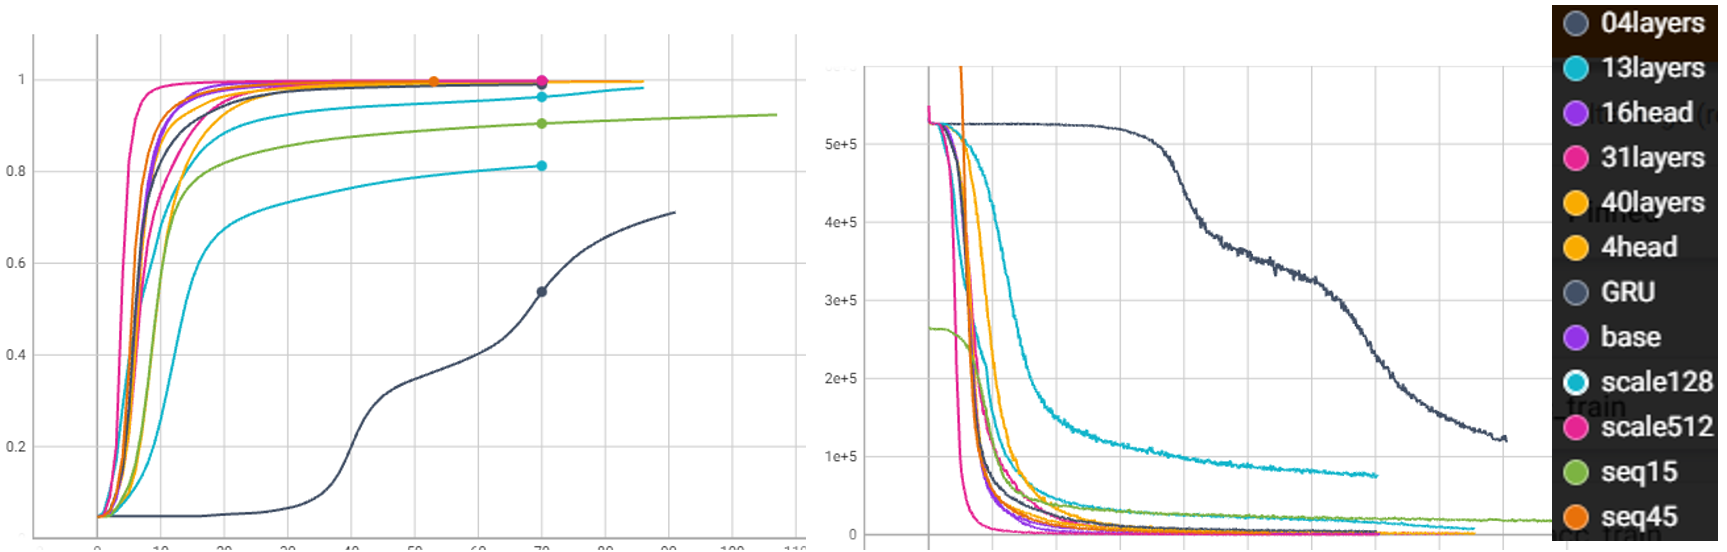
\includegraphics[width=0.9\linewidth]{myReport//figures/componet_curve.png}
    \caption{The training curve of different networks components}
    \label{fig:enter-label}
\end{figure}


\begin{figure}[hbt!]
    \centering
    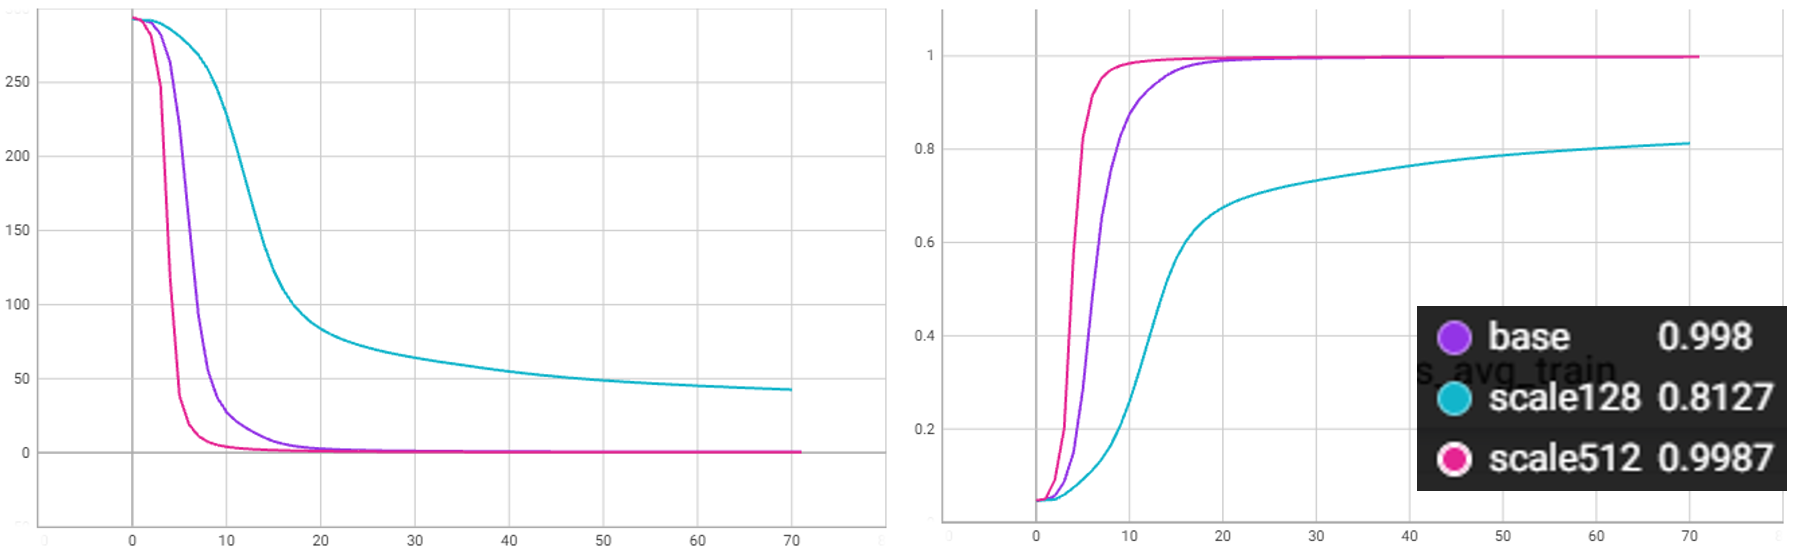
\includegraphics[width=0.9\linewidth]{myReport//figures/scale_curve.png}
    \caption{The training curve of different scale of networks}
    \label{fig:enter-label}
\end{figure}


\noindent\textbf{Scale} \qquad		We trained three different scale of networks based on the number of channels to review the scale required for our task. A large amount of data would require a model with large amount of parameters to fit with. Results shows that network with 128 dimensions only achieve 81.27\% accuracy. The network with 512 dimensions of channels has slightly better performance, but its convergence is faster than the base model. Depends on the result, we assume that the scale of base model can satisfy the requirement of current task, but for future tasks with more complexity, larger scale model is still an option. The larger scale network also show better ability in fitting data.


\begin{figure}[hbt!]
    \centering
    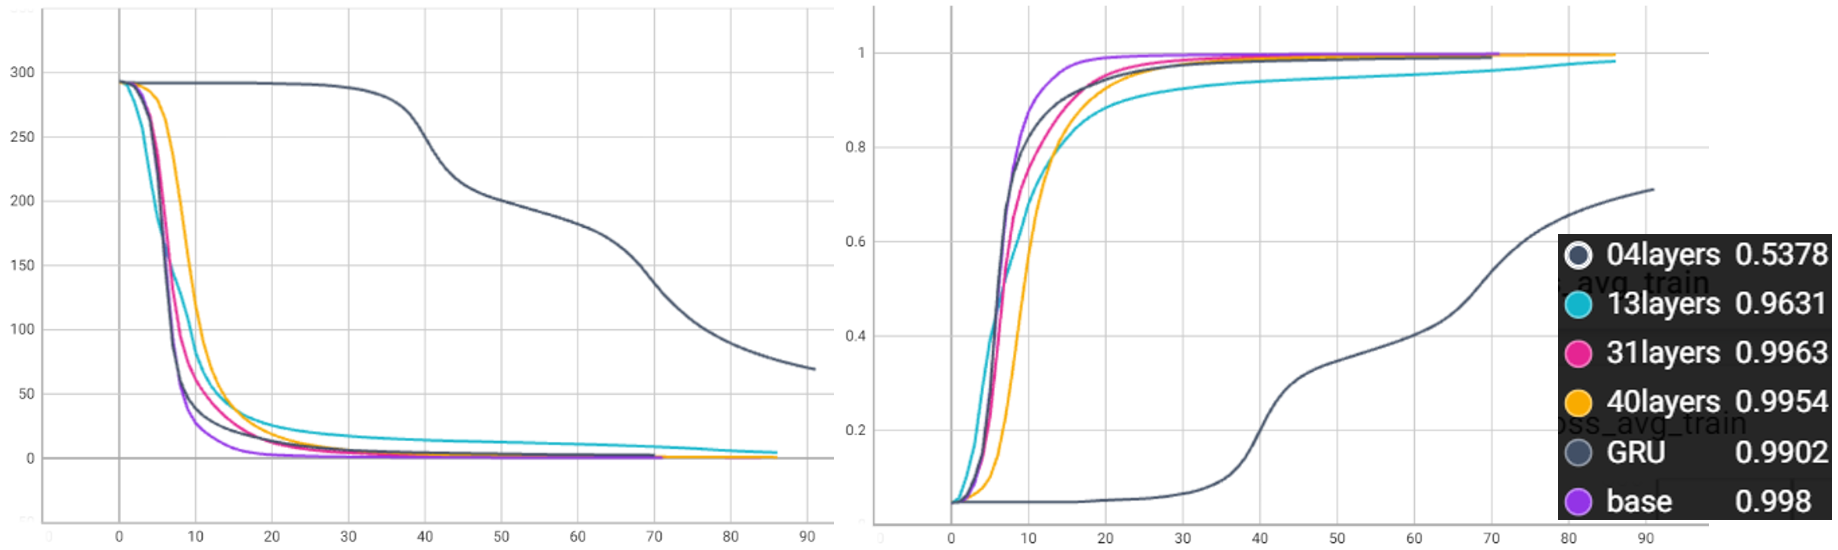
\includegraphics[width=0.9\linewidth]{myReport//figures/layer_curve.png}
    \caption{The training curve of networks with different layers}
    \label{fig:enter-label}
\end{figure}


\noindent\textbf{Type of layers} \qquad		Based on the assumption that LSTM-based networks have better performance in time series analysing task, we trained networks with different types and number of layers. Include different amount of Transformer encoder, LSTM layers, and GRU layers. This experiment is to measure how different types of layers could affect the performance. Results show that the base network still has overall the best performance (99.8\% accuracy). The network with 4 LSTM layers and the network with 3 LSTM and 1 Transformer Encoder layers have similar but slightly lower performance. The network with only 1 LSTM and 3 Transformer Encoder layers has a visible performance drop (96.3\%). The network uses 4 Transformer encoder layers without a LSTM layer has a significant performance drop (53.7\%). The network that replaces LSTM layers with GRU layers also has little performance drop and slower convergence speed. We believe this is the evidence of Recurrent Neural Network, especially LSTM, is the key to our task. The network with at least one LSTM layer all have an overall decent performance. Transformer only network’s converging was slower and didn’t come out with an acceptable result. This also confirm the claim that LSTM has better performance in time series analysis tasks.


\begin{figure}
    \centering
    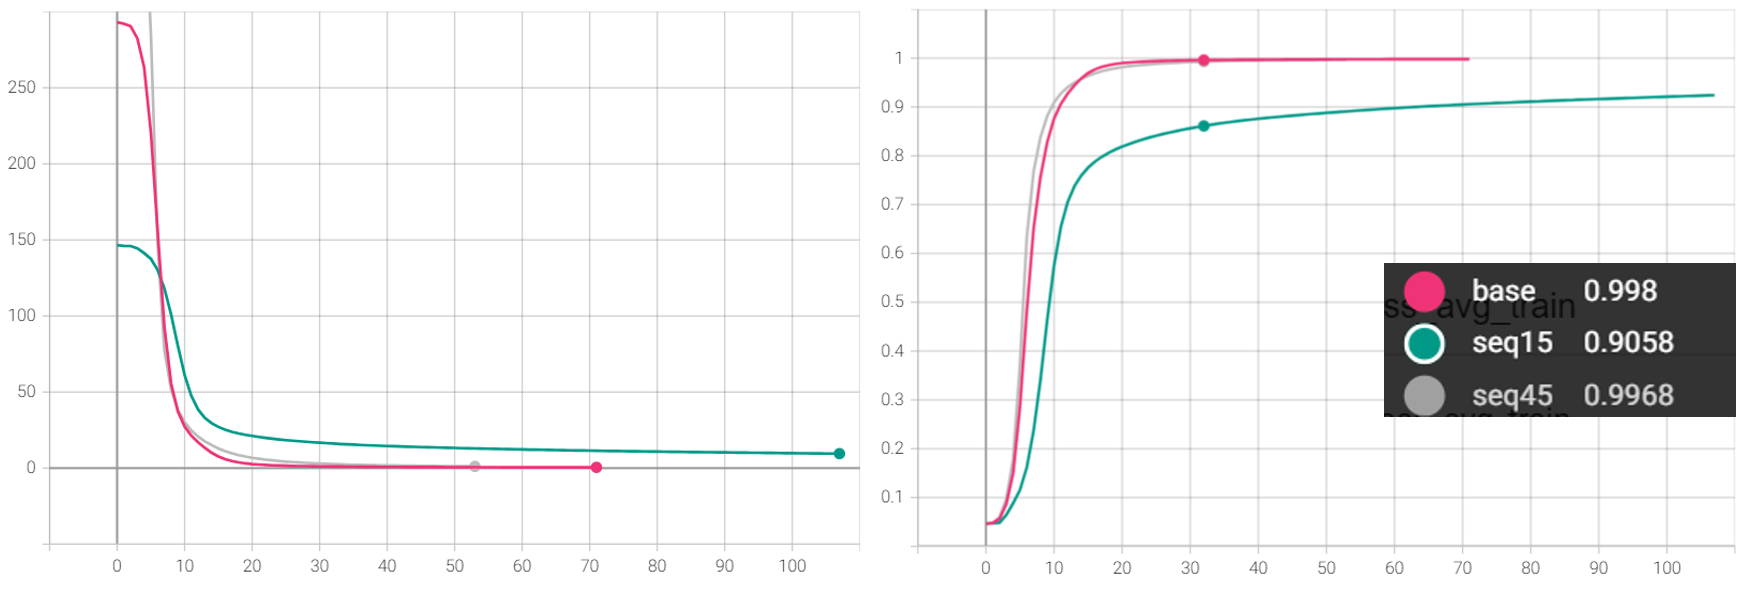
\includegraphics[width=0.9\linewidth]{myReport//figures/seq_curve.png}
    \caption{The training curve of network with different length of sequences}
    \label{fig:enter-label}
\end{figure}


\noindent\textbf{Length of sequences} \qquad		Longer sequences usually lead to more information for analysing, but also harder training. Outside of the base network, we tried training with sequences length 15 and 45. As expected, sequence length 15 training led to a lower accuracy which is 90.6. However, a sequence length 45 didn’t produce improvements over the base model. We assume the reason is more sequence length led to more combination of sequence, which makes the network hard to fit with. Although the result show that sequence with length shorter than 15 start to have performance drop, we still want to optimize the network to make good prediction with shorter sequence.


\section{Multi-Sequence length training}

One of our goals is to analyse how we can recover the key with less information and not be limited to specific length of sequences. For example, a network trained on constant 30 characters length dataset would expect to have reduced performance on the 45 characters length data. Similarly for the shorter sequences like 15 and 5. We want the network to be flexible which means it could maintain decent performance for different length of the data. To tackle these issues, one of the solutions we tried is to train our network with random length data within a pre-defined range. After that, we also test each network’s performance on different lengths. 
During testing, we tested the networks on each different combination of keys. To make the test result reproduceable, we fixed the random seed for PyTorch and Python during testing. 


\begin{figure}
    \centering
    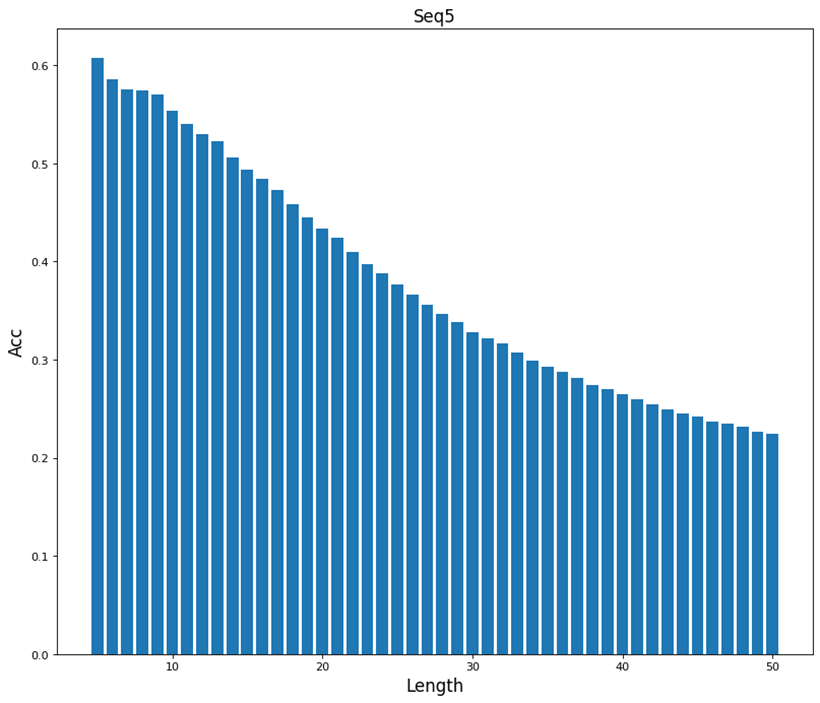
\includegraphics[width=0.7\linewidth]{myReport//figures/seq5_multi_length.png}
    \caption{Accuracy on different length when training data is on fixed length 5.}
    \label{fig:enter-label}
\end{figure}

Figure 14 is the performance of networks trained on length 5 sequences. From the result, we could notice that sequences have around 60\% of accuracy. With testing sequences getting longer, the performance keeps going down.

\begin{figure}[hbt!]
    \centering
    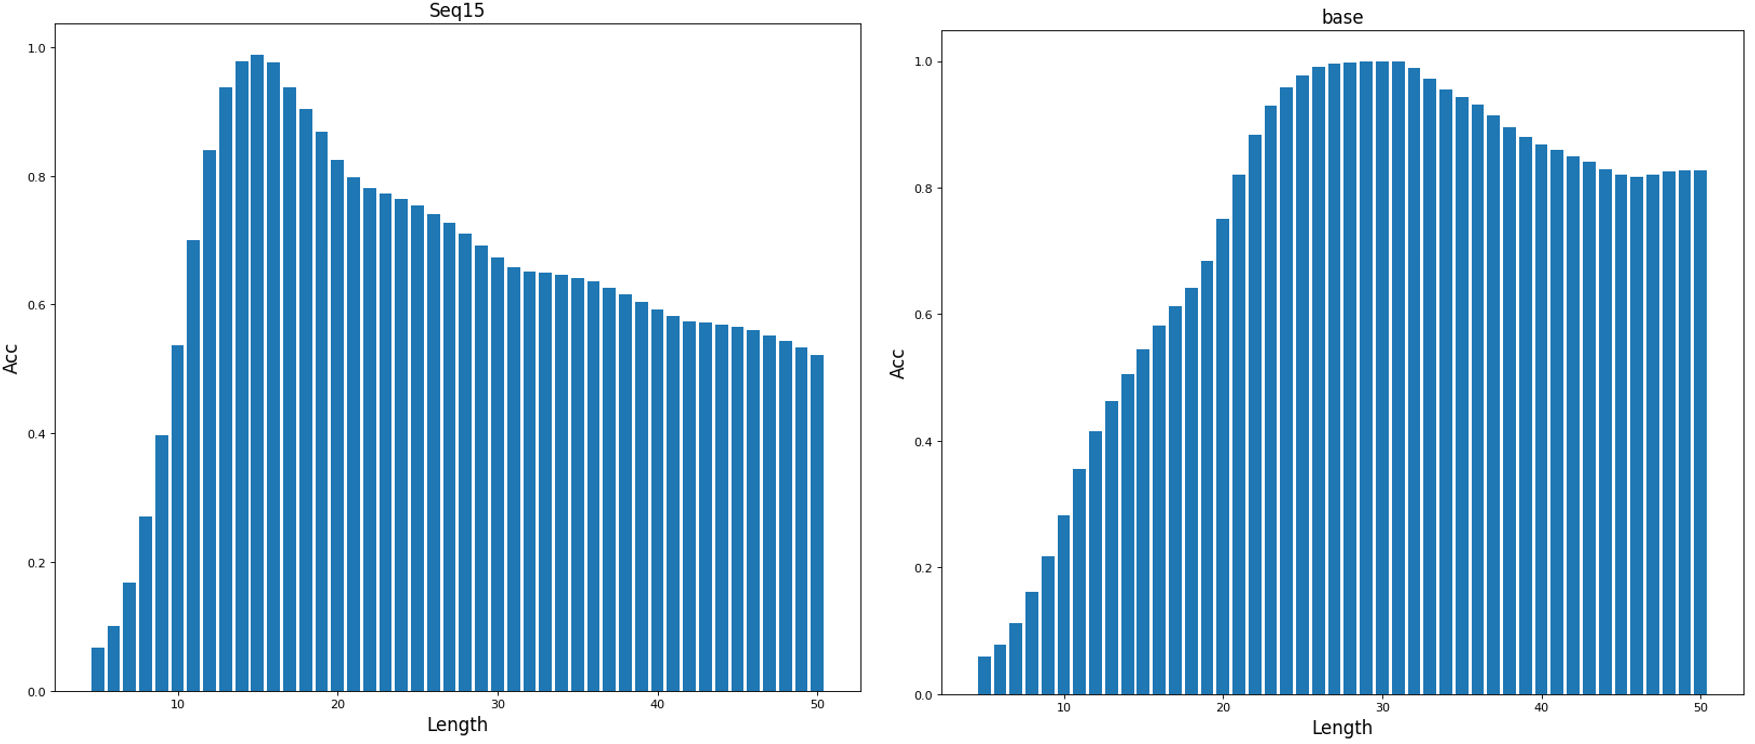
\includegraphics[width=0.75\linewidth]{myReport//figures/seq15_seq45_multi_length.png}
    \caption{Accuracy of network trained with sequence length 15 and sequence length 45.}
    \label{fig:enter-label}
\end{figure}



In Figure 15, we did the same testing on the networks trained on sequences of length 15 and our base model that trained on sequence length 30. We can observe that the tested networks only have good performance at the lengths it trained on. To tackle this issue, we tried to vary the length of sequences we trained on, helping the networks to learn cipher from different length instead of single one. Our implementation is training the network from a range of random length sequences. Constructing a mini batch with different length sequences would require us to use padding values and padding mask. Adding padding values allow us to have different length of sequences in a mini batch and padding mask would help us to only calculate the loss on the non-padded outputs.

\begin{figure}[hbt!]
    \centering
    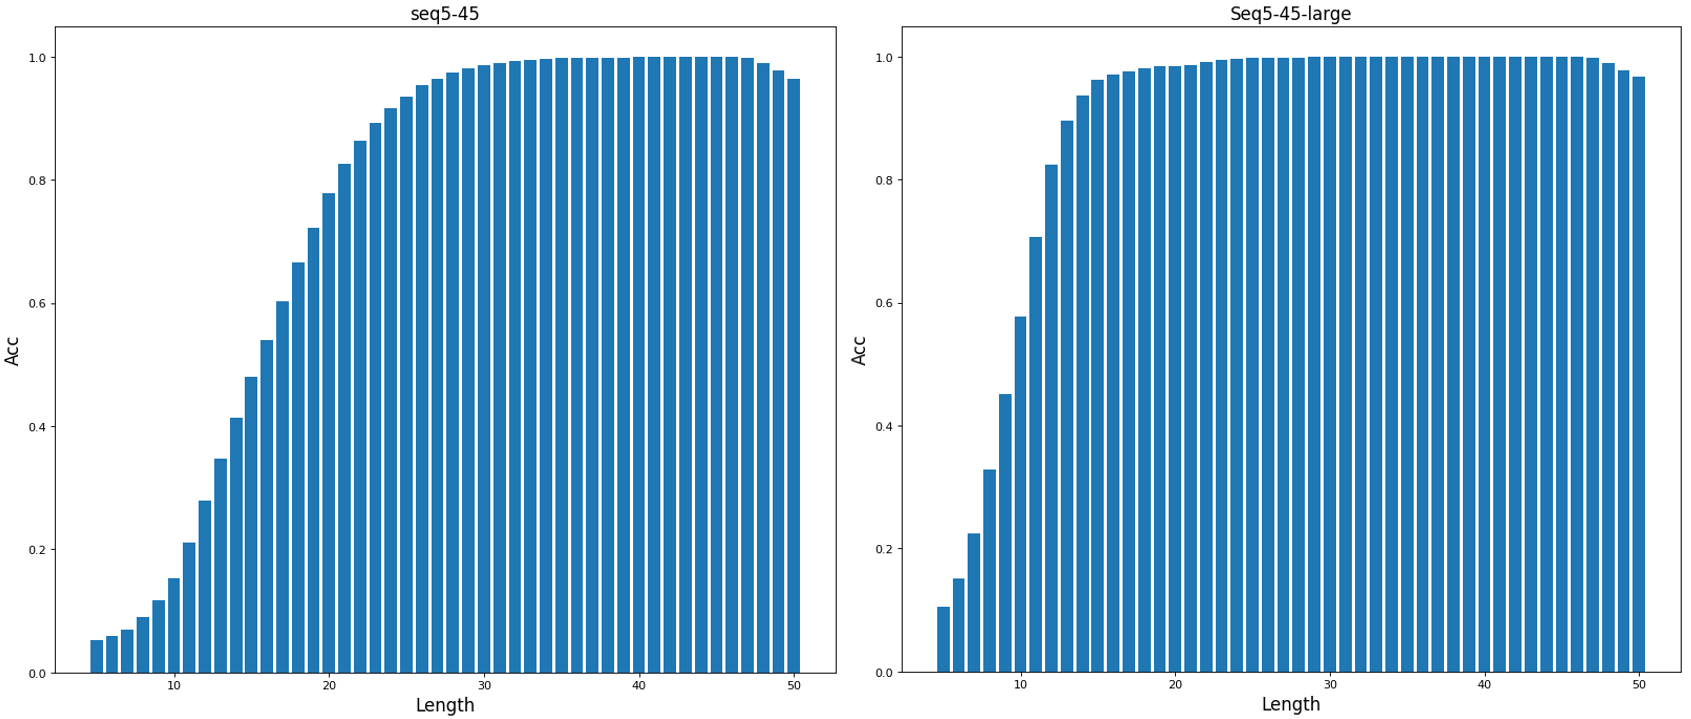
\includegraphics[width=0.75\linewidth]{myReport//figures/different_scale_multi_length.png}
    \caption{Accuracy of base network and large-scale network trained on random sequence length.}
    \label{fig:enter-label}
\end{figure}


By this method, we trained networks with lengths randomly selected between 5 and 45. The graph at left side of Figure 16 shows the accuracy of our base model trained on sequences with length from 5 to 45. We also trained our “larger” model with 512 dimensions inputs with the same setting. Results are listed at the right side of Figure 16. The results shows that networks trained with vary different length sequences could hold their performance on different length’s testing. The large networks also have significantly better overall performance.


\section{Attacking more Enigma's setting}

In the previous experiment, the only variable we introduced is initial state (key bits). Although the network appears to have a very good ability on initial keys, there were Enigma encryption with more variables. Include the setting of rings, rotor types, plugboard setting, and the reflector types. In further experiment, our requirement is implementing the network to predict more variables from Enigma machine and observe its performance on prediction more complex variables. 

Most of the model architectures remains the same as we described in Model architecture part. The original model has a large linear projector layer at the end of network to predict the initial states. We added three more linear projectors to predict the rotor types, ring setting, and plugboard setting. We still used the same method as before, which is the SoftMax Loss to optimize the additional outputs. During the training, we only optimize the part of network that is related to the variables. For example, when we only have one ring setting as a variable, we would only optimize the part of projector that matches with the first ring's setting.

Based on this solution, we tested networks performance under different variables setting. From setting 1 to 2 variables to random to require the networks to predict all settings of Enigma. Most hyperparameters (learning rate, sequence length) remain the same as experiment and result part except the model architecture we used is the second model from Table 1 because this model has overall higher performances than the base model. 

The result showed that the model remains highly accurate when variables didn’t introduce high complexity to the cipher. When we set the type of reflector and the type of first rotor to be random, the complexity of cipher is \(281,216 
 (26^3*2*8)\). In this situation, model could still have significantly above 90 accuracy on predict the rotors and reflector types. When we increase the variable to have two rotors, after 12 hours of training, the network obtains 74\% accuracy initial states and 88\% accuracy on the rotor types. We assume the reason of network taking more time to train and giving lower performance is because of the complexity increased exponentially. The complexity of two random rotors and a random reflector is \(2,249,728 (26^3*2*8^2)\). We expected the network would need more data and parameters to fit with a large complexity cipher like this. In the next stage of experiment, we tried increased the number of random rotor types to 3, which means it has \(17,997,824 (26^3*2*8^3)\) different combination of variables. In this case, the network had failed to fit with the training data. After 12 hours of training, we didn’t observe any sign of converging from the learning curve. 

All the observations above could support our assumption that the network has less ability to analyse cipher with more complexity. We made attempts to increase the performance by tunning part of the hyperparameters. We found that an increase the length of sequence sometimes help increase the performance. We assume the reason is longer sequence contain more information for network to analyse.
